\thispagestyle{empty}
\section{Praktische Durchführung}
\subsection{Hardware}


\pagebreak
\subsection{Docker}
Die Docker Container Technologie wurde 2013 als Open Source Docker Engine eingeführt. Basierend auf Linux Container Konzepten nutz auch Docker Namespaces und C-groups zur Isolierung und Limitierung von Containern.  

\subparagraph{Docker Engine}
Docker ist eine client-server application. Der Docker client kommuniziert mit dem Docker Server oder auch Docker Deamon genannt, der die ganze Arbeit macht. Manchmal wird der Docker Deamon auch Docker Engine genannt. Es ist möglich den Docker Deamon und den Docker client auf dem selben Host laufen zu lassen, oder den localen Docker client mit dem Docker deamon auf einem anderen Host zu verbinden. Die Docker Architektur ist in Abbildung \ref{fig:Docker_Server_Client.PNG} zu sehen\cite{Turnbull2015TheBook}.

\vspace{1em}
\begin{minipage}{\linewidth}
	\centering
	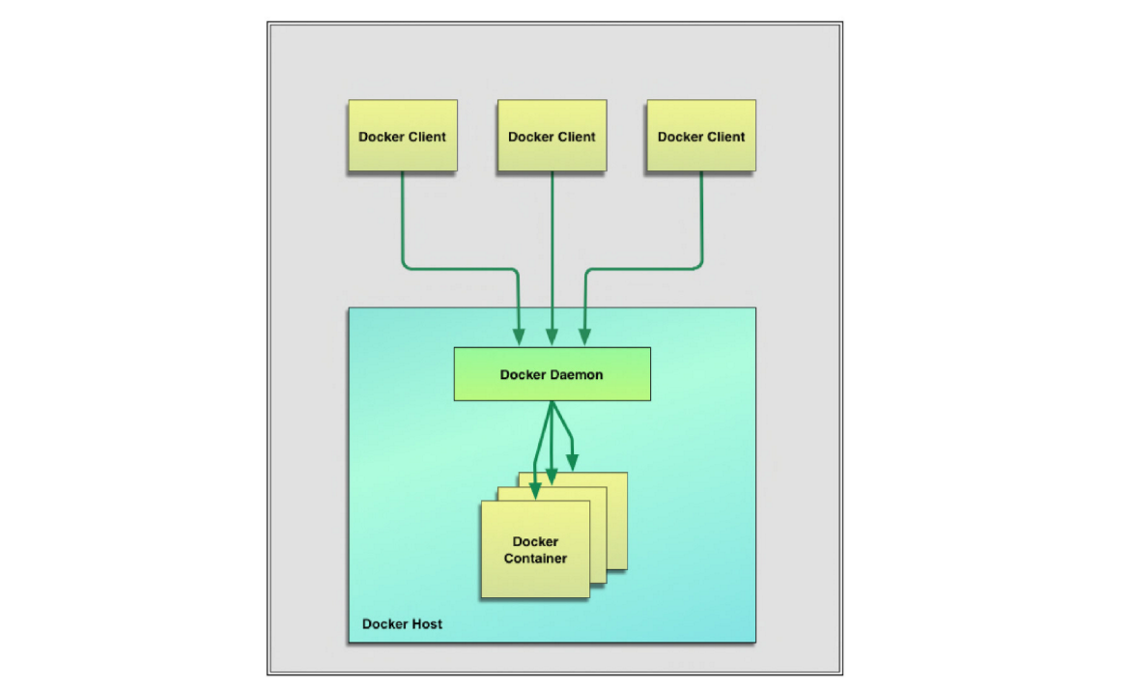
\includegraphics[width=1\linewidth]{pics/Docker_Server_Client.PNG}
	\captionof{figure}[Docker Architektur\cite{Turnbull2015TheBook}]{Docker Architektur}
	\label{fig:Docker_Server_Client.PNG}
\end{minipage}

\subparagraph{Docker Images}
Images sind die Bausteine der Docker welt. Container werden von Images gestartet. Images sind ein mehrschichtiges Format, die unter Verwendung von Union-Dateisystemen Schritt für Schritt anhand unterschiedlicher Instruktionen erstellt werden.Als Quellcode der Container können Images betrachtet werden. Sie sind einfach verschiebbar und können in Registern verwaltet werden.

\subparagraph{Registries}
Docker speichert die erstellten Images in Registern. Es gibt zwei Arten von Registern: Öffentliche und private. Docker verwaltet die öffentlichen Images im Docker Hub\cite{DockerInc.2016DockerHub}. Auf Docker Hub können eigene Images abgespeichert und geteilt werden. Diese Plattform beinhaltet bereits Zehntausende Images die von anderen Leuten erstellt wurden, die für eigene Verwendungen zur Verfügung stehen. Private Images kann man ebenfalls auf Docker Hub abspeichern und niemand außer einem ausgewählten Personenkreis hat zugriff darauf.

\subparagraph{Docker Containers}
Docker unterstützt beim erstellen und ausführen von Containern. Container werden von Images ausgeführt und können einen oder mehrere Prozesse beinhalten. Images können als der aufbau Prozess von Docker gesehen werden und Container als die ausführende Instanz von Docker.

Docker leiht sich das Konzept des standard Schiff Containers die für den Transport von Waren eingesetzt werden, als ein Modell für Docker Container, mit dem Unterschied, dass Docker Container keine Waren sondern Software transportiert. Container können in jeglicher Umgebung ausgeführt werden. Ob auf dem Laptop, nach dem Download von Docker Hub auf einem web server, einem Datenbank- oder auf einem Applikationsserver die Container werden geladen, wie jeder andere Container auch.

\pagebreak

\subsection{Realisierung}
Das oben genannte Szenario wird in Teilprobleme zerlegt und schrittweise zusammengefügt. Im Erste Schritt soll gezeigt werden Wie sich der Ressourcenverbrauch eines Containers erhöht und wo eventuelle grenzen der verwendeten Hardware liegen. Im Linux-File-System ist es möglich über die PID eines vorhandenen Prozesses die Cgroup herauszufinden zu der ein Prozess gehört. Zur erinnernung, jede Cgroup ist für die Ressourcen Begrenzung, Priorisierung, Abrechnung und Kontrolle aller Prozesse zuständig die unter ihr erstellt wurden. Unter einem Kontrollregister im Linux-Kernel kann die Summe der verwendeten Ressourcen aller unter einer Cgroup laufenden Prozesse zur Laufzeit ausgelesen werden. Was zu der Idee führte, einen neuen Docker-Container zu erstellen, in diesem einen Prozess mit einem malloc() befehlt in einer Endlosschleife auszuführen und die menge des allokierten Speichers der cgroup auszuwerten. Ein malloc() befehl 

\subparagraph{Test01}
Auf Docker-Hub wurde ein geeignetes Image ausgesucht und für diese Zwecke erweitert. Beim ausführen des Image ist nun ein Docker-Container erstellt worden. Ressourcen Limits konnten ebenfalls vor dem starten des Containers eingestellt werden. Für den ersten Start des Docker-Containers sind allerdings noch keine Begrenzungen des Speichers nötig, da es in erster Linie um die Auswirkung des ausgeführten C-Programms auf die Ressourcenverwaltung im Container geht. Der verwendete C-Code den der Prozess ausfüht, ist in Listing \ref{01mem} zu sehen. Ein erstelltes Skript verwendet die beim Start erzeugte PID, findet die Cgroup in der der Prozess ausgeführt wird und schreibt die ausgelesenen Messdaten in ein txt-File. Die Messdaten wie Clock-Time in Nanosekunden und Speicherverbrauch in Bytes werden für die Auswertung verwendet.

\vspace{1em}
\lstinputlisting[caption=Einfacher C-Code, label=01mem, basicstyle=\ttfamily\scriptsize]{code/01mem.txt}

\subparagraph{Erwartungshaltung Test 01}
Falls das Skript die Messwerte in ungefähr gleichmäßig schnellen Abständen liefert, und die Speicher Allocationen gleich schnell ablaufen, wird eine Gerade Funktion hypothetisch erwartet, die gleichbleibend schnell ansteigt und wenn nicht mehr genug Speicher im System vorhanden ist beendet wird.

\vspace{1em}
\begin{minipage}{\linewidth}
	\centering
	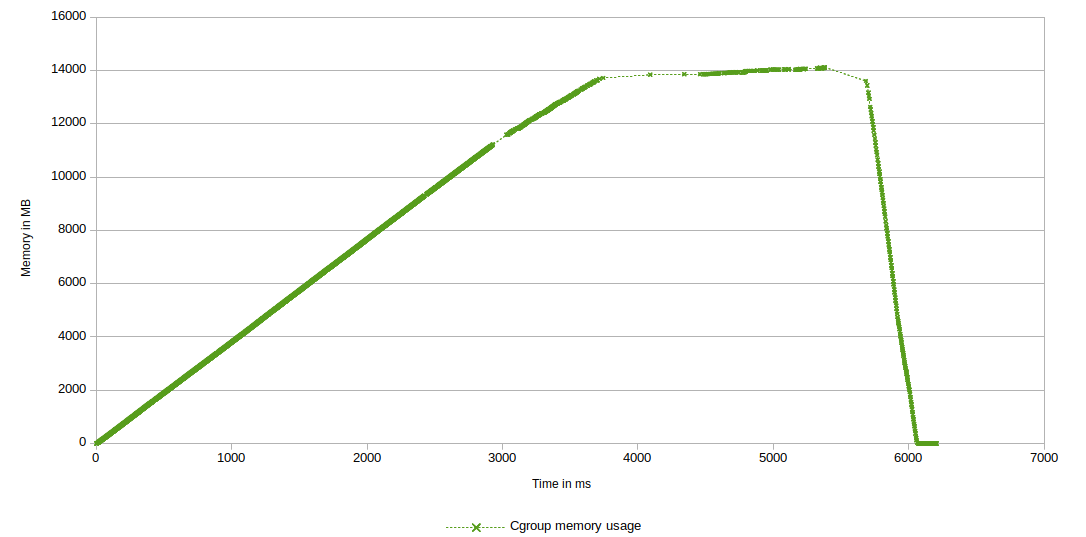
\includegraphics[width=1\linewidth]{pics/001_mem_usage_No_Limit_Cgroup_RDY_FOR_USE.png}
	\captionof{figure}[Speicher Verbrauch Cgroup Ohne Limit]{Memory usage Cgroup no Limit}
	\label{fig:001_mem_usage_No_Limit_Cgroup_RDY_FOR_USE}
\end{minipage}

\subparagraph{Ergebnis Test01}
In Abbildung \ref{fig:001_mem_usage_No_Limit_Cgroup_RDY_FOR_USE} ist wie erwartet eine gleichmäßige Steigung erkennbar. Bei ca. 13900MB Allociertem Speicher bricht die Wachstumsrate ein. An diesem Punkt ist der insgesamt 16GB große Arbeitsspeicher größtenteils Ausgeschöpft. Ein paar MegaByte konnten vom Betriebssystem für den dauerhaft nach mehr Speicher verlangendem Prozess gefunden werden. Bei knapp über 14000MB wurde der OOM-Killer eingeschaltet um wichtigere Prozesse zu schützen, und der Container wurde beendet.

\subparagraph{Test02}
Im nächsten Schritt wird der Verlauf einer Cgroup näher betrachtet, bei der ein Speicherlimit festlegt wird, das nicht überschritten werden soll (Hard-Limit). Um dieses Limit zu erstellen, wurde das Image entsprechend angepasst und das Speicherlimit auf 8200 Megabyte gesetzt. Das in Listing \ref{01mem} vorgestellte Programm wurde nochmals ausgeführt.

\subparagraph{Erwartungshaltung Test 02}
Da nun ein Hard-Limit eingerichtet ist wird prognostiziert, dass die Cgroup mit der gleichen Geschwindigkeit wie in Abbildung \ref{fig:001_mem_usage_No_Limit_Cgroup_RDY_FOR_USE} bis zum gesetzten Limit ansteigt und dieses nicht überschreiten wird. 

\vspace{1em}
\begin{minipage}{\linewidth}
	\centering
	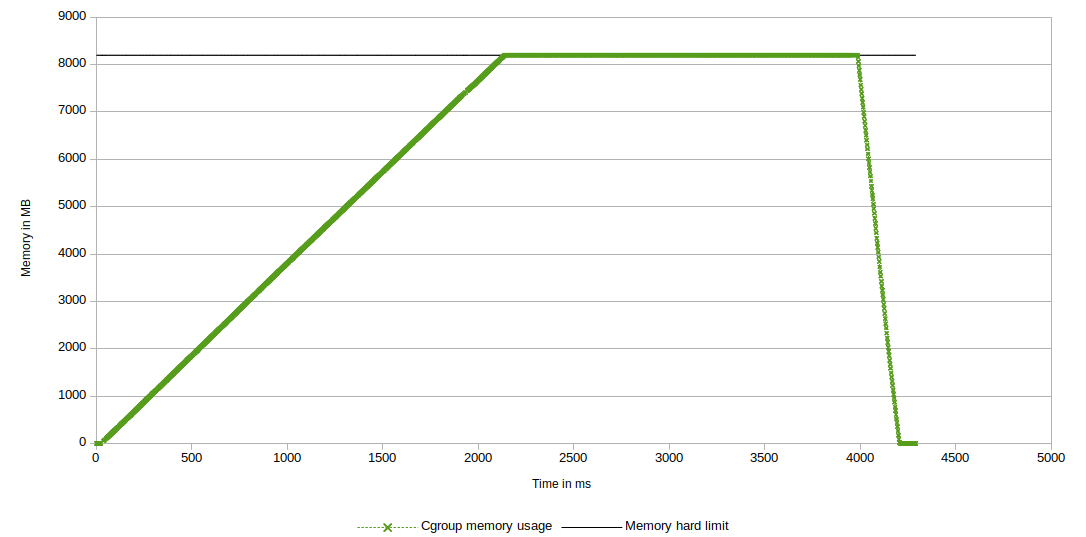
\includegraphics[width=1\linewidth]{pics/002_mem_usage_8200mb_limit_Cgroup_RDY_FOR_USE.png}
	\captionof{figure}[Speicher Verbrauch Cgroup 8200MB Limit]{Memory usage Cgroup 8200MB Limit}
	\label{fig:002_mem_usage_8200mb_limit_Cgroup_RDY_FOR_USE}
\end{minipage}

\subparagraph{Ergebnis Test02}
Mit einer Allocations Rate von ca. 4000MB/S auf dem ausgeführten Host-System ändert sich an der Speicher Zugriffsrate nichts, das Limit von 8200MB wurde erfolgreich eingehalten und der Prozess wurde wieder vom Betriebssystem beendet.

Schon fast Vorbildlich hält sich die Cgroup an das gesetzte Limit. Da stellt sich die Frage "wie kann man sich eine Cgroup anschaulich vorstellen, was zeigt sie an, wie weit kann sie verwendete Ressourcen der einzelnen Prozesse verfolgen?". 


Die Cgroup ist wie eine Box. Die Größe der Box wird bei der Erstellung des Containers festgelegt. In Abbildung \ref{fig:002_mem_usage_8200mb_limit_Cgroup_RDY_FOR_USE} waren es 8200MB. Der Füllstand der Box setzt sich aus den verwendeten Ressourcen aller in der Box ausgeführten Prozesse zusammen. Wenn ein Prozess wie in Abbildung \ref{fig:002_mem_usage_8200mb_limit_Cgroup_RDY_FOR_USE} die Komplette Box ausfüllt und weiter darüber hinaus ragen würde, wäre die Box nur in der Lage den Füllstand bis zu Ihrer Maximalgröße von 8200 MB wiederzuspiegeln. Der Überlaufende teil des Prozesses kann von der Cgroup nicht erkannt werden.

\subparagraph{Test03}
Nach dem Einblick der Anzeigemöglichkeiten einer Cgroup liegt es nun nahe, den Prozess der durch das Ausführen des oben genannten C-Codes entsteht, genauer anzusehen. Der Test wird mit einer Skript Erweiterung um die Anzahl der verwendeten Memory-Pages des Prozesses wiederholt. Die Anzahl an verwendeten Memory-Pages in einem laufenden Prozess, kann ebenfalls im Linux-Kernel ausgelesen werden. Eine Memory-Page ist 4KB groß und wird für die Auswertung mit der Anzahl an Memory-Pages multipliziert.

\subparagraph{Erwartungshaltung Test 03}
Wenn die Memory-Page Größe multipliziert mit der Anzahl an verwendeten Memory-Pages genau dem entspricht, was die Cgroup an Speicher Allocation ausgibt, sollten beide Graphen bis zum erreichen des Limits parallel verlaufen.

\vspace{1em}
\begin{minipage}{\linewidth}
	\centering
	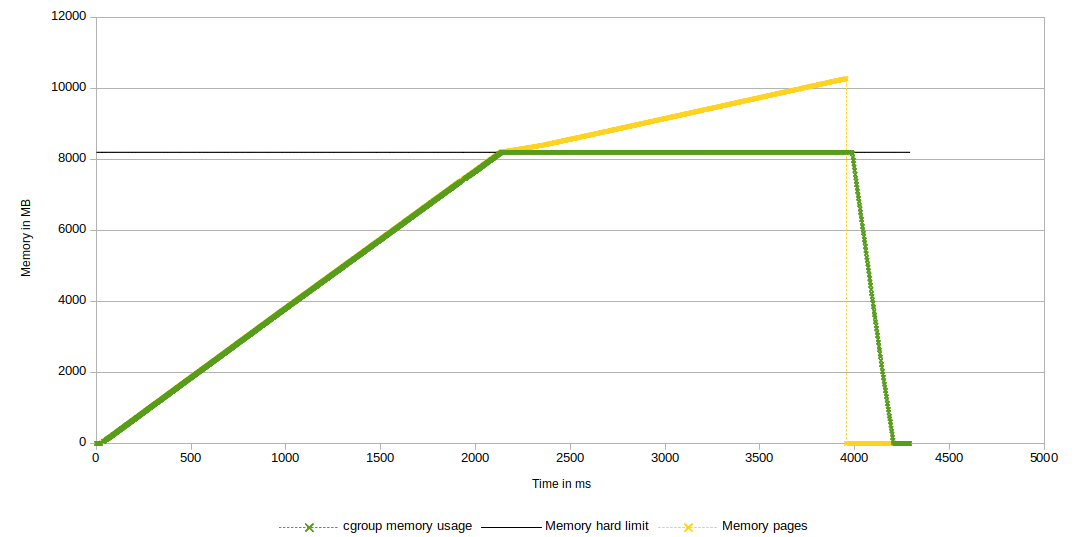
\includegraphics[width=1\linewidth]{pics/003_mem_usage_8200mb_limit_Cgroup_Pages_RDY_FOR_USE.png}
	\captionof{figure}[ Endlosschleife Malloc]{Memory usage Cgroup Memory pages 8200MB Limit Endlosschleife Malloc}
	\label{fig:003_mem_usage_8200mb_limit_Cgroup_Pages_RDY_FOR_USE}
\end{minipage}

\subparagraph{Ergebnis Test03}
Deutlich zu erkennen sind die exat aufeinanderliegeneden Messwerte der Cgroup und der Memory Pages. Ab 8200MB schießen die allocierten Memory Pages bis ca 10200MB über das Limit hinaus. Erkennbar ist auch die geringere Allocationsrate sofort nach dem Überlauf auf 2000MB/s fällt. Komplett ignoriert wurde das Limit allerdings nicht. Verglichen mit Abbildung \ref{fig:001_mem_usage_No_Limit_Cgroup_RDY_FOR_USE} war noch genügend Speicher im System vorhanden. Wieso wurde der Prozess dann überhaupt schon beendet, warum konnte er über das Limit hinaus allokieren, wie verhält sich ein Container wenn er nur ein wenig über das Limit geht, wie wirkt sich das auf andere Container im System aus?

Eine Antwort ist das sogenannte "Paging". Beim Paging werden Allokierte aber aktuell nicht verwendete Memory Pages vom Arbeitsspeicher auf den Massenspeicher geladen. In Abbildung \ref{fig:003_mem_usage_8200mb_limit_Cgroup_Pages_RDY_FOR_USE} ist nach 8200MB die Trennung zwischen der Gelben Linie "Memory pages" und der Grünen Linie "cgroup memory Usage" zu erkennen. Zu diesem Zeitpunkt hat das Betriebssystem mit dem Paging begonnen und lädt von dem Prozess allokierte Pages in den Massenspeicher. Die Tatsächliche menge an von der Cgroup Allokiertem Arbeitsspeicher auf der Hardware bleibt gleich. Die Gelbe Linie zeigt die Summe aller vom Prozess Allokierten Memory Pages, folglich auch den auf den Massenspeicher Ausgelagerten Anteil. Die Steigung der Gelben Linie ist einfach nachzuvollziehen. Wegen der Erhöhten Anforderung an das I/O System was das Paging zu verantworten hat, verringert sich die Allocationsrate beim überschreiten des Limits. Der überlauf von ca 2GB stimmt mit dem 2GB Paging Limit überein.

\subparagraph{Test03,5}
zur Abklärung und Überprüfung des Paging Limits, empfiehlt sich den Test aus Abbildung \ref{fig:010_mem_usage_8200mb_limit_Container03_undContainer04_RDY_FOR_USE_Focu} mit Erweiterung von Memory Pages zu wiederholgen.

\subparagraph{Erwartungshaltung Test03,5}
Es wurden ca 14000MB beim ersten Testdurchlauf allokiert. Mit dem zusätzlichen Paging Limit von 2GB sind die Memory Pages auf ca 16000MB zu schätzen. Ein Identischer cgroup Graph wird nicht erwarten, da der Arbeitsspeicherverbrauch des Betriebsstems von mehreren Faktoren abhängt. Doch der Unterschied zwischen Cgruop memory Usage und Memory Pages sollte bei etwa 2GB liegen. 

\vspace{1em}
\begin{minipage}{\linewidth}
	\centering
	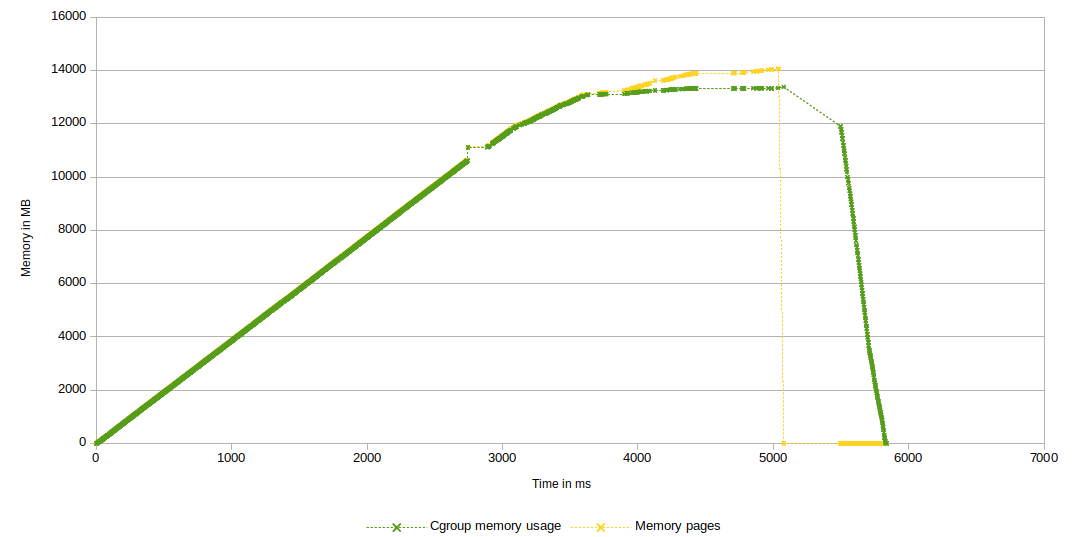
\includegraphics[width=1\linewidth]{pics/001,5_mem_usage_No_Limit_Cgroup_Pages_RDY_FOR_USE.png}
	\captionof{figure}[Speicher Verbrauch Cgroup 8200MB Limit]{Memory usage Cgroup 8200MB Limit}
	\label{fig:001,5_mem_usage_No_Limit_Cgroup_Pages_RDY_FOR_USE.png}
\end{minipage}

\subparagraph{Ergebnis Test03,5}
In Abbildung \ref{fig:001,5_mem_usage_No_Limit_Cgroup_Pages_RDY_FOR_USE.png} sind die 2GB unterschied zwischen "Cgroup memory usage" und den "Memory Pages" offensichtlich nicht erreicht worden, was mehrere Gründe haben kann. Möglich ist eine zusätzliche Speicheranforderung des Betriebssystems während der Prozess in der Paging Phase war und zum früheren Absturz geführt hat. Dieser Effekt wird in dieser Arbeit aus Zeitgründen nicht näher untersucht. Auch des unterschiedlich schnelle Abfallen der Linien beim beenden des Prozesses wird nicht näher beleuchtet. 



\subparagraph{Test04}
Um auf die große Ziel hin zu arbeiten, wird nun ein Container der für eine gewisse Zeitspanne läuft und etwas mehr als das gesetzte Limit allociert benötigt. Der in Listing \ref{01mem} gezeigte C-Code wurde zu Listing \ref{02mem} verändert. 

\vspace{1em}
\lstinputlisting[caption=einfacher C-Code, label=02mem, basicstyle=\ttfamily\scriptsize]{code/02mem.txt}

\subparagraph{Erwartungshaltung Test 04}
Nachdem der Malloc(sizeof(int)*1024) Befehl jetzt 2200000 mal ausgeführt wird, ein Integer 4Byte groß ist *1024 sind 4KB pro Ausführung, sollte der Graph der Memory Pages bei etwa 8600MB verharren und 60 Sekunden diesen Wert halten.

\vspace{1em}
\begin{minipage}{\linewidth}
	\centering
	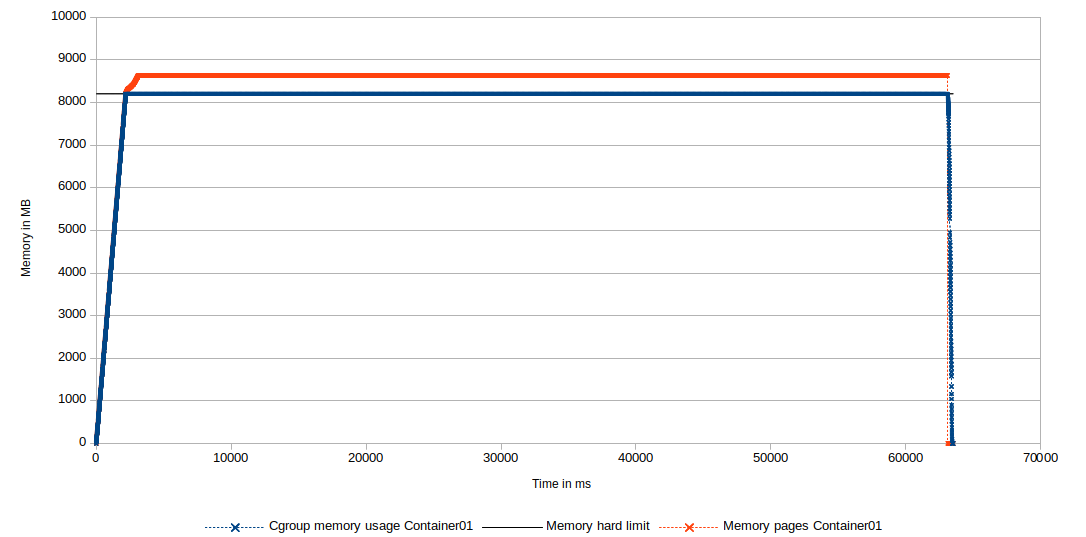
\includegraphics[width=1\linewidth]{pics/004_mem_usage_8200mb_limit_Container01_Basis_RDY_FOR_USE.png}
	\captionof{figure}[Speicher Verbrauch Cgroup 8200MB Limit]{Memory usage Cgroup 8200MB Limit}
	\label{fig:004_mem_usage_8200mb_limit_Container01_Basis_RDY_FOR_USE}
\end{minipage}

\subparagraph{Ergebnis Test04}
Wie in Abbildung \ref{fig:004_mem_usage_8200mb_limit_Container01_Basis_RDY_FOR_USE} zu entnehmen, ist es möglich für einen längeren Zeitraum über das Limit hinaus Ressourcen zu Allokieren. Durch die lange Ausführungszeit gleichbleibender Ressourcen ist es jetzt möglich den Einfluss von Container untereinander zu untersuchen. Dieser Container wird von nun an als Container01 bezeichnet.

\subparagraph{Test05}
Im Ablauf des folgenden Tests wird zuerst Container01 gestartet, und während der Laufzeit wird Container02 ebenfalls eingeschaltet. Der Container02 wird zum besseren Verständnis in Abbildung \ref{fig:005_mem_usage_8200mb_limit_Container02_Basis_RDY_FOR_USE_FOCUS} nochmals in skalierter Umgebung dargestellt. 


\vspace{1em}
\begin{minipage}{\linewidth}
	\centering
	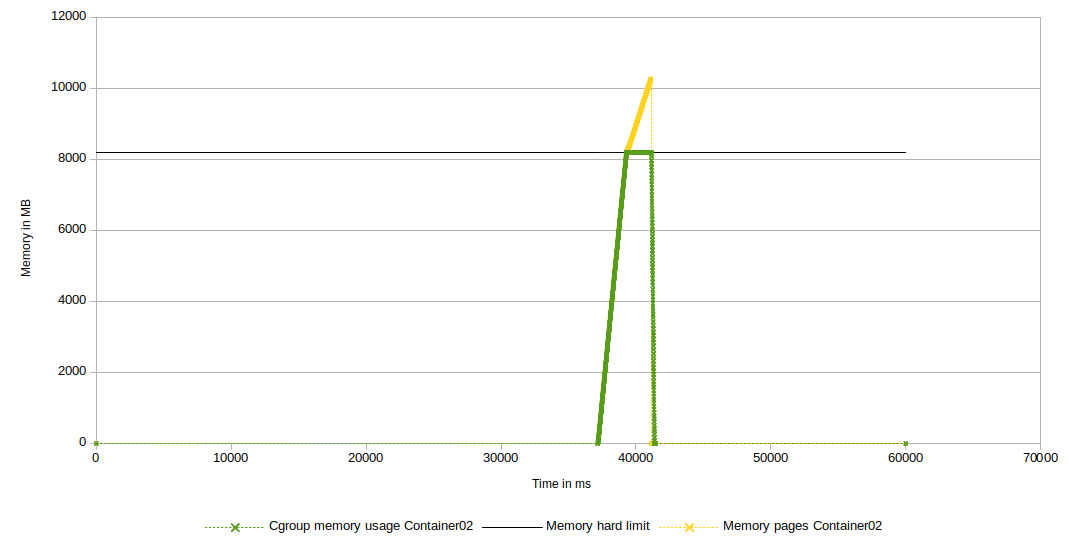
\includegraphics[width=1\linewidth]{pics/005_mem_usage_8200mb_limit_Container02_Basis_RDY_FOR_USE_FOCUS.png}
	\captionof{figure}[Speicher Verbrauch Cgroup 8200MB Limit]{Memory usage Cgroup 8200MB Limit}
	\label{fig:005_mem_usage_8200mb_limit_Container02_Basis_RDY_FOR_USE_FOCUS}
\end{minipage}

\subparagraph{Erwartungshaltung Test 05}
Die verwendbaren Systemressourcen liegen nach Abbildung \ref{fig:001_mem_usage_No_Limit_Cgroup_RDY_FOR_USE} bei etwa 14000MB. Allein Container01 verwendet schon ca. 8600MB der gesamten Summe, was die Deckelung von Container02 auf 8200MB rein rechnerisch unnötig macht, da dieser Wert mit den verwendbaren Ressourcen nicht erreicht werden kann. Somit wird Container02 frühzeitig beendet werden. 

\vspace{1em}
\begin{minipage}{\linewidth}
	\centering
	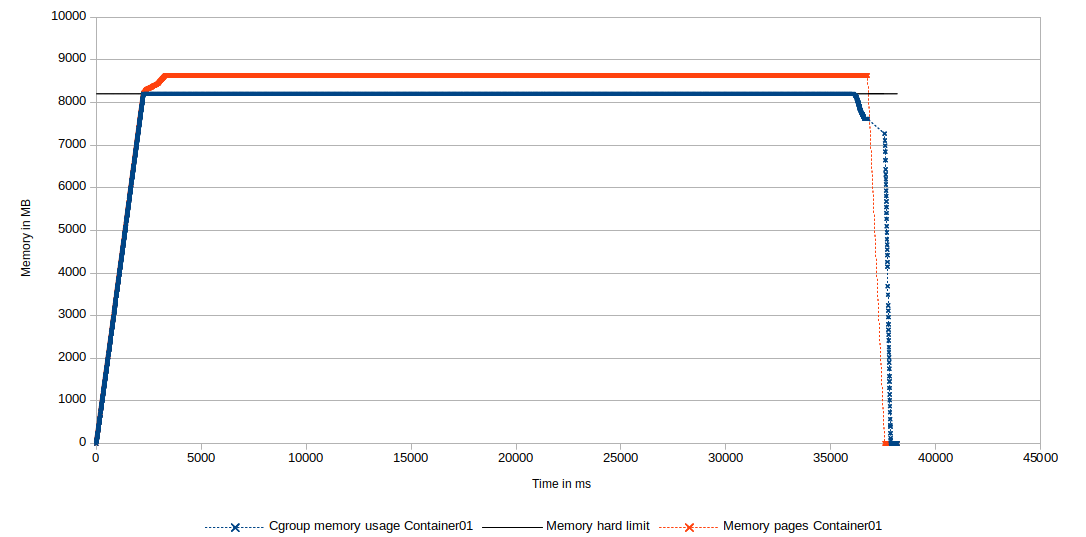
\includegraphics[width=1\linewidth]{pics/006_mem_usage_8200mb_limit_Container01_mit_ipact_RDY_FOR_USE.png}
	\captionof{figure}[Speicher Verbrauch Cgroup 8200MB Limit]{Memory usage Cgroup 8200MB Limit}
	\label{fig:006_mem_usage_8200mb_limit_Container01_mit_ipact_RDY_FOR_USE}
\end{minipage}

\subparagraph{Ergebnis Test05}
Nach Betrachtung von Abbildung \ref{fig:006_mem_usage_8200mb_limit_Container01_mit_ipact_RDY_FOR_USE} ist zu erkennen, dass Container01 nicht nach ca. 63 Sekunden geplant beendet wurde, sondern schon etwa nach ca 38 Sekunden. Was die oben genannte Hypothese nicht erfüllt.

Abbildung \ref{fig:007_mem_usage_8200mb_limit_Container01_und_Container02_RDY_FOR_USE} zeigt was passiert ist. kurz nach dem Start von Container 02 als dieser ca 5100MB Speicher Allociert hat, wird Container 01 beendet. Container 02 überschreitet das Limit von 8200MB nach ca. 41 Sekunden und wird nach ca. 42,5 Sekunden ebenfalls beendet.

\vspace{1em}
\begin{minipage}{\linewidth}
	\centering
	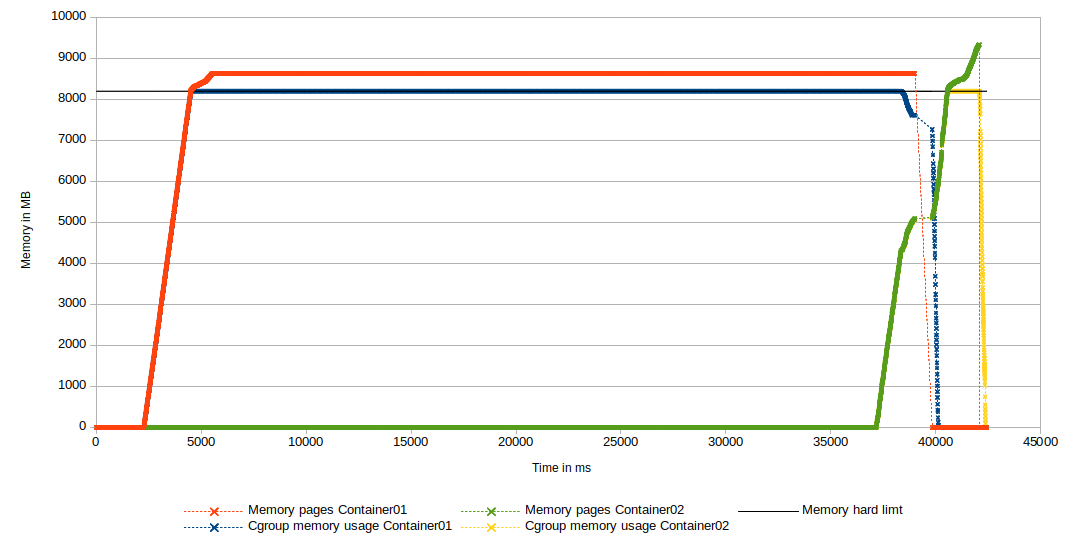
\includegraphics[width=1\linewidth]{pics/007_mem_usage_8200mb_limit_Container01_und_Container02_RDY_FOR_USE.png}
	\captionof{figure}[Speicher Verbrauch Cgroup 8200MB Limit]{Memory usage Cgroup 8200MB Limit}
	\label{fig:007_mem_usage_8200mb_limit_Container01_und_Container02_RDY_FOR_USE}
\end{minipage}

Deutlicher zu sehen ist in Abbildung \ref{fig:008_mem_usage_8200mb_limit_Container01_und_Container02_RDY_FOR_USE_FOCUS} wie die einzelnen Graphen verlaufen. Am auffälligsten ist die große Lücke (mit gestrichelten Linien gekenzeichnet) in der Mitte der Abbildung. Eine Lücke entsteht, wenn über mehrere Millisekunden keine Messwerte vom Skript erfasst werden konnten. In diesem Fall ist das auf eine Systemüberlastung zurück zu führen, welche durch die Überlastung des Arbeitsspeichers und die dadurch eingeleiteten Systemreaktionen entstanden ist. 

\vspace{1em}
\begin{minipage}{\linewidth}
	\centering
	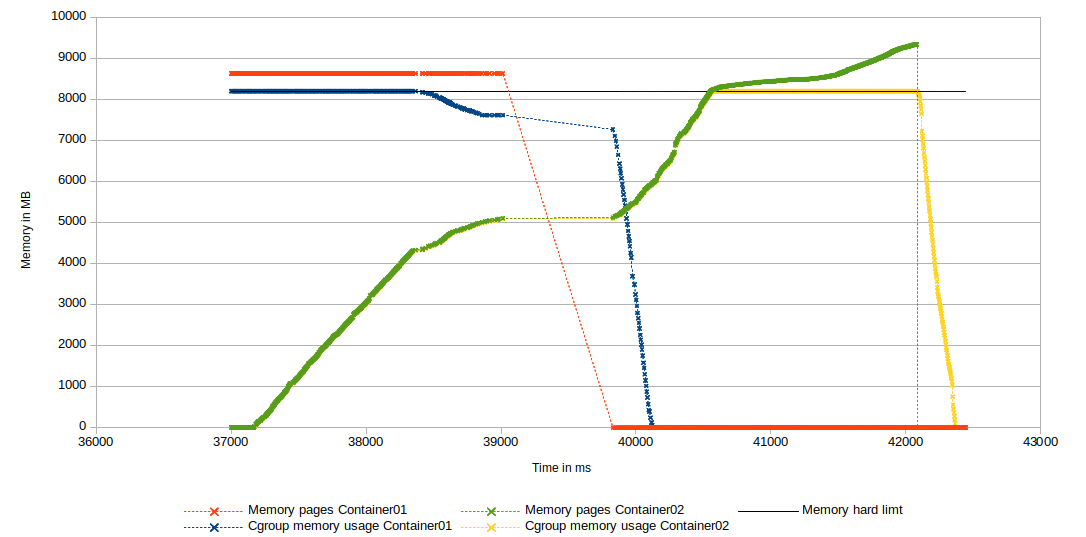
\includegraphics[width=1\linewidth]{pics/008_mem_usage_8200mb_limit_Container01_und_Container02_RDY_FOR_USE_FOCUS.png}
	\captionof{figure}[Speicher Verbrauch Cgroup 8200MB Limit]{Memory usage Cgroup 8200MB Limit}
	\label{fig:008_mem_usage_8200mb_limit_Container01_und_Container02_RDY_FOR_USE_FOCUS}
\end{minipage}



Eine der Systemreaktionen ist das sogenannte "Paging". Beim Paging werden Allokierte aber aktuell nicht verwendete Memory Pages vom Arbeitsspeicher auf den Massenspeicher geladen. An der Blauen Linie "Cgroup memory usage Container01" in Abbildung \ref{fig:008_mem_usage_8200mb_limit_Container01_und_Container02_RDY_FOR_USE_FOCUS} ist nach ca. 38.5 Sekunden ein Abwertstrend zu erkennen. Zu diesem Zeitpunkt hat das Betriebssystem mit dem Paging begonnen und lädt von der Cgroup allokierte Pages in den Massenspeicher. Die Tatsächliche menge an von der Cgroup Allokiertem Arbeitsspeicher wird weniger. Die Rote Linie "Memory pages Container01" zeigt die Summe aller vom Prozess Allokierten Memory Pages, folglich auch den auf den Massenspeicher Ausgelagerten Anteil. Der Verlauf der Grünen Linie "Memory pages Container02" ist einfach nachzuvollziehen. Wegen der Erhöhten Anforderung an das I/O System was das Paging zu verantworten hat, verringert sich die Allocationsrate. Nach dem beenden von Container01, was auch das Paging beendet, verläuft die Steigung ähnlich schnell wie kurz nach dem Start des Prozesses. 

\subparagraph{Test06}
Bisher wurden Container betrachtet, die sich nicht an das vorgegebene Limit gehalten haben. Im folgenden gilt es zu zeigen, dass auch bei "gutartigen" Containern, also Container welche sich immer unter dem vorgegebenen Limit befinden, ähnliche Effekte auftreten. Für den folgenden Testdurchlauf wurde der in Listing \ref{02mem} gezeigte C-Code verwendet und Zeile 8 durch Listing \ref{03mem} ersetzt. Zuerst startet Container03 der den neu generierten C-Code ausführt. Während der 60 Sekunden Sleep Phase startet Container04 auch mit dem in Container03 verwendeten Code.

\vspace{1em}
\lstinputlisting[caption=einfacher C-Code, label=03mem, basicstyle=\ttfamily\scriptsize]{code/03mem.txt}

\subparagraph{Erwartungshaltung Test 06}
Durch die Änderung auf 2048000 Wiederholungen des Malloc Befehls, wird Container03 bis ca. 8000MB Speicher Allokieren. Nach dem Start von Container04 wird ein ähnlicher Graphen verlauf erwartet wie im vorherigen Test. Da das gesetzte Hard Limit bei 8200MB nicht überschritten wird, sollten die Linien "Cgroup memory usage Container04" und "Memory Pages Container04" identische über die Lebensdauer des Containers verlaufen.

\vspace{1em}
\begin{minipage}{\linewidth}
	\centering
	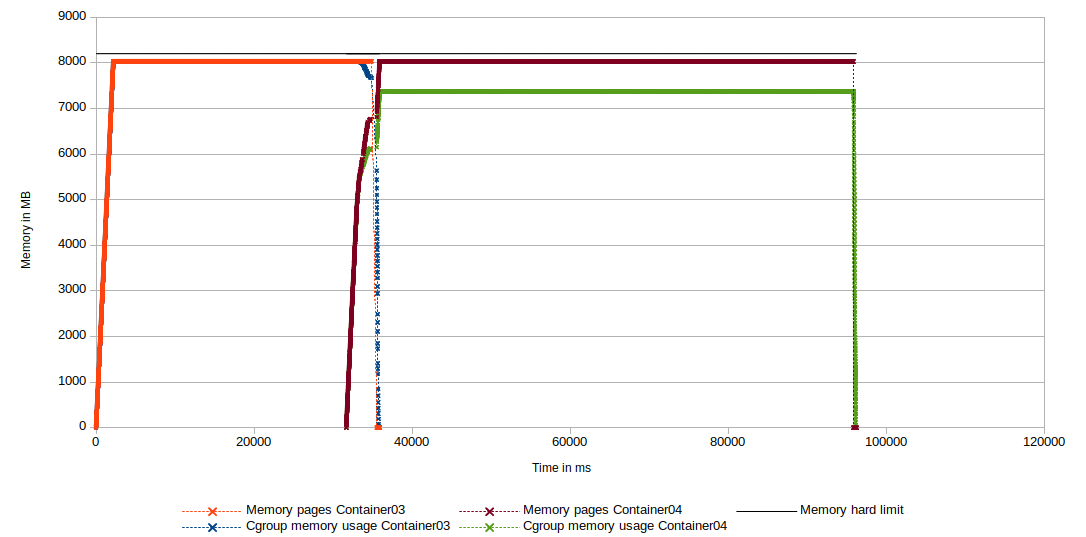
\includegraphics[width=1\linewidth]{pics/009_mem_usage_8200mb_limit_Container03_undContainer04_RDY_FOR_USE.png}
	\captionof{figure}[Speicher Verbrauch Cgroup 8200MB Limit]{Memory usage Cgroup 8200MB Limit}
	\label{fig:009_mem_usage_8200mb_limit_Container03_undContainer04_RDY_FOR_USE}
\end{minipage}

\subparagraph{Ergebnis Test06}
Der Verlauf von Container03 in Abbildung \ref{fig:009_mem_usage_8200mb_limit_Container03_undContainer04_RDY_FOR_USE} war Container01 in Abbildung \ref{fig:007_mem_usage_8200mb_limit_Container01_und_Container02_RDY_FOR_USE} sehr ähnlich. Betrachtet man in Abbildung \ref{fig:010_mem_usage_8200mb_limit_Container03_undContainer04_RDY_FOR_USE_Focu} die Blaue Linie "Cgroup memory usage Container03" und die Dunkel Rote Linie "Cgroup memory usage Container04" fällt auf, dass das Betriebssystem nach ca 33,5 Sekunden mit dem Paging angefangen hat und Einfluss auf die Cgroups beider Container nimmt. Das Resultat ist vergleichbar mit dem aus Abbildung \ref{fig:008_mem_usage_8200mb_limit_Container01_und_Container02_RDY_FOR_USE_FOCUS}.  

\vspace{1em}
\begin{minipage}{\linewidth}
	\centering
	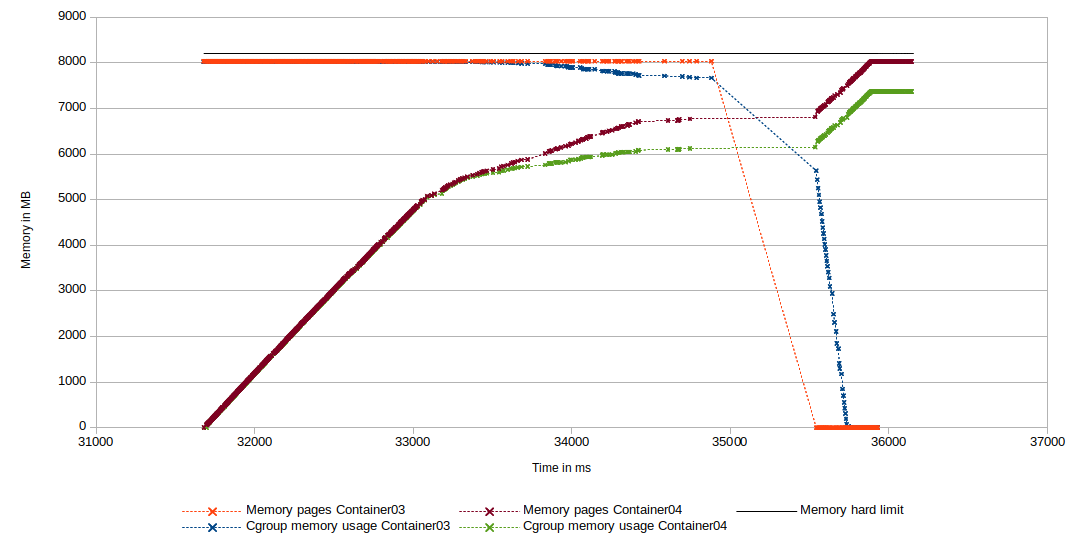
\includegraphics[width=1\linewidth]{pics/010_mem_usage_8200mb_limit_Container03_undContainer04_RDY_FOR_USE_Focus.png}
	\captionof{figure}[Speicher Verbrauch Cgroup 8200MB Limit]{Memory usage Cgroup 8200MB Limit}
	\label{fig:010_mem_usage_8200mb_limit_Container03_undContainer04_RDY_FOR_USE_Focu}
\end{minipage}

Container04 verläuft bei der Allokation unter dem gesetzten Limit wegen des Unterschied von der in Abbildung \ref{fig:009_mem_usage_8200mb_limit_Container03_undContainer04_RDY_FOR_USE} Grün dargestellte Linie "Cgroup memory usage Container04" und der Dunkelroten Linie "Memory pages Container04" nicht wie erwartet. . In Abbildung\ref{fig:007_mem_usage_8200mb_limit_Container01_und_Container02_RDY_FOR_USE} vor der Lücke war nur Die Blau dargestellte Linie "Cgroup memory usage Container01" vom Paging betroffen und die Parallel zur grün verlaufende Gelbe Linie "Cgroup memory usage Container02" zeigte keine Anzeichen von Paging. Auch an dieser Stelle wird auf den Seiteffekt verursacht durch das Paging aus Zeitgründen nicht weiter eingegangen.

Es wurde gezeigt, dass ein neu ausgeführter Container mit im Linux-Kernel implementierten Mechanismen in der Lage ist, einen bereits bestehend Container zu beenden und dann auf dessen Ressourcen zuzugreifen.



\pagebreak 
